\chapter{Fundamentals}

\section{Electric Mobility}
\label{ch:Introduction:sec:Electric Mobility}

E-mobility, short for "electromobility," refers to the use of \acrfull{ev} and other electric-powered transportation options as an alternative to conventional vehicles that run on \acrfull{ice}. As key component of the global effort to tackle climate change and achieve sustainable transportation solutions, it targets the reduction of greenhouse gas emissions, decrease dependence on fossil fuels, and mitigate the environmental impact of transportation \cite{kathiresh_e-mobility_2022}.

\subsection{Electric Vehicles}
\label{ch:Introduction:sec:Electric Mobility:Electric Vehicles}
As a fundamental cornerstone of e-mobility, \acrfullpl{ev} describe automobiles, which are powered by one or more electric engines drawing draw energy from onboard batteries or similar energy sources. \acrshortpl{ev} come in various forms, including \acrfullpl{bev}, \acrfullpl{phev}, and \acrfullpl{hev}. \acrshortpl{bev} run solely on electric power, while \acrshortpl{phev} combine an electric motor with an internal combustion engine, and \acrshortpl{hev} use both power sources but cannot be plugged in for charging \cite{kathiresh_e-mobility_2022}.

\subsection{Charging Infrastructure}
\label{ch:Introduction:sec:Electric Mobility:ssec:Charging Infrastructure}

Beside \acrshortpl{ev} the necessary charging infrastructure is one of the critical components of e-mobility. To support the widespread adoption of \acrfullpl{ev}, a robust network of \acrfullpl{cs} is essential. These stations can vary from residential charging points to public \acrfullpl{cs} installed in parking lots, streets, and commercial areas. Different charging levels exist, ranging from slow Level 1 chargers (typically used at home) to rapid \acrshort{dc} fast chargers found in public locations for quick charging \cite{afshar_literature_2020}.

On a more general level, \acrfullpl{cs} could be differentiated into the following classes:

\begin{figure}[!ht]
    \centering
    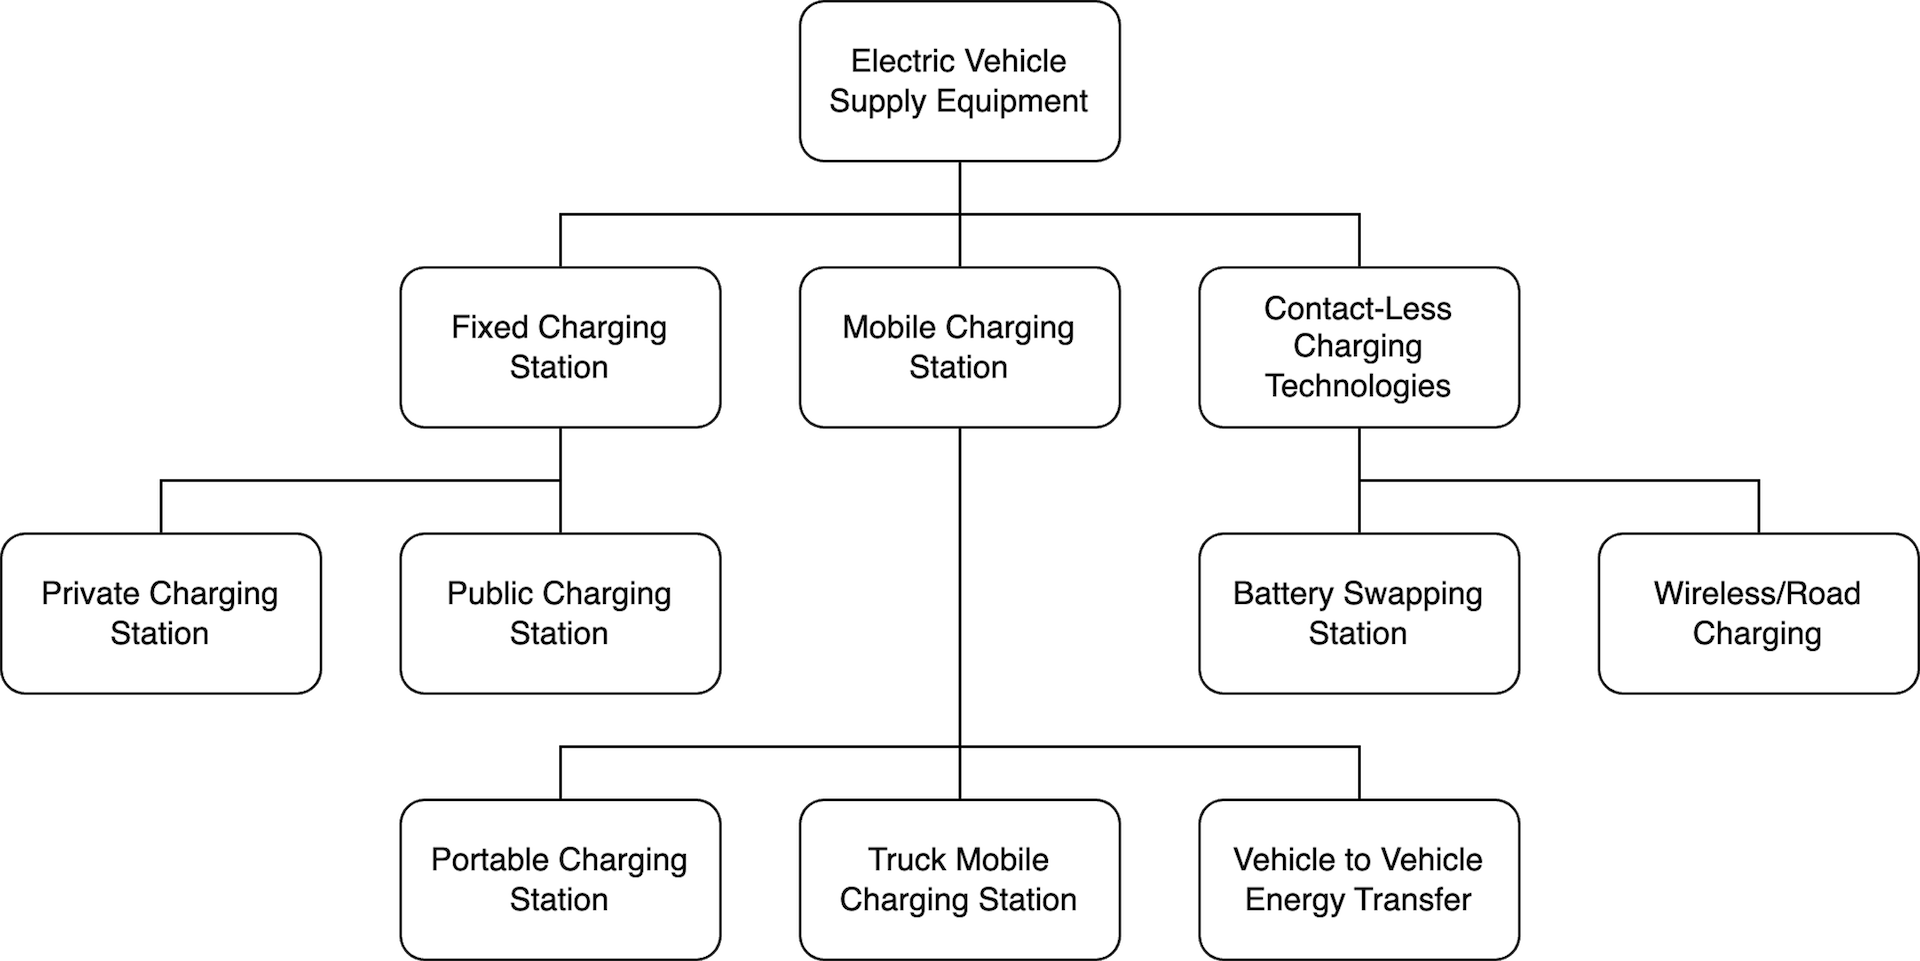
\includegraphics[scale=0.4]{resources/images/main/1_fundamentals/ChargingStationClassification.png}
    \caption{Approach of a classification of charging stations based on \cite{afshar_literature_2020}}
    \label{fig:enter-label}
\end{figure}

A more fine-granular definition is \acrfull{evse}, which refers to the infrastructure and hardware used for charging. It encompasses all the components and systems necessary to supply electric power from an electrical grid to the battery of an \acrfull{ev}, allowing it to charge and store energy for driving. Typically, it consists of the following components:

\begin{enumerate}
    \item \textbf{\acrfull{cs}}\\The physical structure or unit where the \acrshort{ev} is connected to receive electricity. \acrfullpl{cs} can vary in size and complexity, ranging from small wall-mounted units designed for home use to more extensive public \acrfullpl{cs} found in parking lots, shopping centers, and along roads.
    \item \textbf{Connector or Charging Cable}\\The cable that connects the \acrshort{ev} to the \acrfull{cs}. It contains plugs on both ends, one connecting to the vehicle's charging port and the other to the \acrfull{cs}'s outlet.
    \item \textbf{\acrfull{pms}}\\An integral part of the \acrshort{evse} that regulates the flow of electricity from the grid to the vehicle's battery. It ensures safe and efficient charging, managing the power level based on the vehicle's battery capacity and the grid's capacity.
    \item \textbf{Communication and Control System}\\This system enables communication between the \acrshort{ev}, the \acrfull{cs}, and the grid. It allows data exchange regarding charging status, electricity prices, user authentication, and other relevant information.
    \item \textbf{Payment and Authentication System}\\For public \acrfull{cs}, a payment and authentication system may be integrated into the \acrshort{evse}. This system verifies the user's identity, authorizes the charging session, and processes payment for the electricity consumed.
    \item \textbf{Safety Features}\\ \acrshort{evse} is equipped with safety features to protect users, the vehicle, and the surrounding environment. This includes features like ground fault protection, overcurrent protection, temperature monitoring, and emergency shut-off capabilities \cite{littlefuse_designing_2020}.
\end{enumerate}

Furthermore, a differentiation into specialised types of \acrshort{evse}, categorized based on the charging power and speed they offer, is possible \cite{spendiff-smith_different_2022}.

\begin{enumerate}
    \item \textbf{Level 1 Charging}\\The most basic form of \acrshort{evse}, Level 1 charging uses a standard household 120-volt AC outlet to charge the vehicle. It is typically the slowest charging option and is suitable for overnight charging at home.
    \item \textbf{Level 2 Charging}\\Level 2 charging utilizes a 240-volt AC power source, commonly found in residential and commercial settings. It provides faster charging compared to Level 1 and is commonly used for home charging setups and public charging stations.
    \item \textbf{\acrshort{dc} Fast Charging (Level 3 Charging)}\\\acrshort{dc} fast charging is the fastest charging option and operates at a higher voltage, directly charging the vehicle's battery with \acrshort{dc} power. It is commonly used in public fast-charging stations and can provide a significant amount of charge in a short time.
\end{enumerate}

\subsection{Battery Technology}
\label{ch:Introduction:sec:Electric Mobility:ssec:Battery Technology}

To store the energy required for powering electric vehicles, batteries are inevitable in the further development and acceptance of the \acrfullpl{evu} in case of range axiety and countering insufficient public charging infrastructure \cite{basmadjian_interoperable_2019}. Advancements in this technology regarding the increase in range of \acrshortpl{ev} and the reduction of charging times in combination with cost-effectiveness . Lithium-ion batteries are the most common type used in electric vehicles today, but research is ongoing to develop new battery chemistries with improved performance and longevity.

\subsection{Communication protocols}
\label{ch:Introduction:sec:Electric Mobility:ssec:Communication protocols}

To provide a general interface for information exchange between the \acrfull{cs} and the \acrfull{ev} and their users the \acrfull{oca} developed the so called \acrfull{ocpp} as standard communication protocol. It supports a standard set of functions, which could be used by the \acrfull{csms} to manage \acrshort{csms}.

\subsubsection{Open Charge Point Protocol}
\label{ch:Introduction:sec:Electric Mobility:ssec:Communication protocols:sssec:Open Charge Point Protocol}

The \acrfull{ocpp} is an industry-standard communication protocol used in \acrshort{ev} charging infrastructure to enable communication between \acrshort{evse} and \acrshort{csms}. \acrshort{ocpp} is designed to provide interoperability and seamless integration between different charging station vendors and network operators, ensuring that EV drivers can charge their vehicles at any compatible charging station. Therefore, it is an open protocol and not not proprietary to any specific manufacturer or organization. It is maintained by the \acrfull{oca}, a consortium of \acrshort{ev} charging infrastructure stakeholders, ensuring that it remains a collaborative and evolving standard \cite{noauthor_ocpp_nodate-1}.

\acrshort{ocpp} could be described as a client/server architecture. The \acrshort{evse} in this model acts as the client, while the \acrshort{csms} serves as the server. The server responds to the client's requests and manages the charging processes accordingly. This request-response model, where the client sends requests to the server, and the server responds with the appropriate information or action enables real-time communication between the \acrfull{cs} and the connected \acrfull{cms}.

As an interface for communication, two different types of protocols are used. On the one side, the WebSocket protocol for bidirectional communication, providing a persistent connection between the \acrshort{evse} and the \acrshort{cms} and allowing a faster and more efficient communication. \acrfull{soap} on the other side, is used for one-way communication.

To differentiate between particular feature sets, the \acrshort{ocpp} is versioned. The versions are illustrated as floating point numbers, which are increasing based on major or minor releases. The most recent protocol versions are \acrshort{ocpp} 1.5, \acrshort{ocpp} 1.6, \acrshort{ocpp} 2.0 and often include enhancements, additional features and bug fixes based on the increased part of the versioning.

Afterwards a collection of relevant \acrshort{ocpp} operations based on \cite{noauthor_ocpp_nodate-1}:

\begin{enumerate}
    \item \textbf{Boot Notification}\\The charging station sends a boot notification to the \acrshort{cms} when it starts up or connects to the network. This notification allows the \acrshort{cms} to identify and track the status of the charging station.
    \item \textbf{Authorize}\\Before starting a charging session, the \acrshort{evu} RFID card or other identification is sent to the central system for authorization. The \acrshort{cms} checks the driver's credentials and responds with an authorization status.
    \item \textbf{Start Transaction}\\After successful authorization, the \acrshort{cms} sends a start transaction request to initiate the charging process. The \acrshort{cs} acknowledges the request, and the charging session begins.
    \item \textbf{Meter Values}\\During the charging session, the \acrshort{cs} periodically sends meter values to the \acrshort{cms}, providing real-time information on charging status, power consumption, and other relevant data.
    \item \textbf{Stop Transaction}\\When the charging session is complete or terminated, the charging station sends a stop transaction request to the \acrshort{cms}, indicating the end of the charging process. Based on the gathered meter values, the \acrshort{cms} responds with transaction-related information, such as the total energy consumed and the charging cost.
    \item \textbf{Status Notification}\\The \acrshort{cs} may send status notifications to the \acrshort{cms} to update the current state of the charging station, such as "Available," "Charging", "Reserved", or "Faulted".
    \item \textbf{ReserveNow}\\In case a user needs an available connector on a \acrshort{cs}, he could send a "ReserveNow" request via the \acrshort{cms} to the \acrshort{cs}, which reserves one specific or at least on connector on the station for a specified duration. This connector changes from status "Available" to "Reserved" and only the user assigned to the deposited RFID card is able to charge at the connector or \acrshort{cs}.
    \item \textbf{Cancel Reservation}\\For cancelling the created reservation the user could manually send a request with the assigned reservation id to the \acrshort{cms} to free the connector again. Otherwise, the \acrshort{cs} will notify the \acrshort{cms}, if the reservation is expired.   
\end{enumerate}

\subsubsection{Open Charge Point Interface}
\label{ch:Introduction:sec:Electric Mobility:ssec:Communication protocol:sssec:Open Charge Point Interface}
\acrfull{ocpi} is an open standard protocol designed for communication between \acrshort{cs} and \acrshort{csms} or \acrshort{cpo}. It facilitates interoperability and seamless communication among various charging network operators, enabling \acrshort{ev} drivers to access charging infrastructure from different providers using a unified and standardized approach. 

Key Components of \acrshort{ocpi} are the defined endpoints, used for communication between \acrshort{cs} and \acrshortpl{cms}. These endpoints include for example functionalities like location discovery, charge point data, authorization, charging sessions, and error handling. For integrating \acrshort{ocpi} into existing software systems it is heavily based on the paradigm of \acrfull{rest}. This allows communication via standard HTTP methods utilizing \acrfull{json} as data format for transmitting information. 

The listing below provides a short overview of available features and functionalities provided by \acrshort{ocpi} \cite{noauthor_ocpiocpi_2023}:

\begin{enumerate}
    \item \textbf{Location Discovery}\\Charging networks can exchange information about available charging locations, providing details such as location coordinates, charging station types, and status.
    \item \textbf{Charge Point Data}\\Charging station data, including information on charging station availability, status, and pricing, can be accessed through OCPI.
    \item \textbf{Charging Sessions}\\OCPI supports real-time information about ongoing charging sessions, including start time, energy consumed, and current charging status.
    \item \textbf{Authorization and Authentication}\\OCPI allows EV drivers to be authenticated and authorized to access charging services through their respective CPO accounts or other authentication methods.
    \item \textbf{Remote Start/Stop Charging Sessions}\\OCPI enables the remote start and stop of charging sessions, allowing EV drivers to initiate charging sessions via their mobile apps or other remote means.
    \item \textbf{Tariff Information}\\Charging networks can share pricing and tariff information, providing transparency to EV drivers about the cost of charging at different locations.
\end{enumerate}

\subsection{Smart Charging}
\label{ch:Introduction:sec:Electric Mobility:ssec:Smart Charging}

The technology of smart charging or intelligent charging, is a systematic approach, which optimizes the charging process to be more efficient, cost-effective, and environmentally friendly. The concept of smart charging revolves around utilizing information and communication technologies to monitor and regulate the charging of electric vehicles, taking into account factors such as electricity demand, grid capacity, renewable energy availability, and preferences of single users.

One of the primary goals of this methodology is to balance the demand on the underlying grid. Charging large numbers of electric vehicles simultaneously, especially during peak hours could result in increased electricity costs or potential blackouts. Therefore, smart charging takes the current load of the grid into account and adjust the possible charging rates based on the given constraints. Prevention of overloading the grid and optimizing the use of available energy are only two side effects resulting out of this approach. 

Furthermore, the integration of \acrfull{tou} electricity plans offer different electricity rates at different times of the day. During peak hours the rates increase and gets lower during off-peak hours. This could be used to initiate scheduled charging when electricity prices are lower, saving the money for the \acrshortpl{evu} and reducing the strain on the grid. 

This effect could be doubled by leveraging real-time data on renewable energy availability, such as solar and wind power. Smart Charging systems could prioritize charging when enough electricity out of renewables is available. This not only reduces greenhouse gas emissions associated with charging \acrshortpl{ev} but also maximizes the utilization of clean and sustainable energy sources.

Beside the unidirectional charging method originally called \acrfull{v1g}, the approach of \acrfull{v2g} enables smart charging systems to charge bidirectionally between the \acrshortpl{ev} battery and the grid. During times of high demand, \acrshortpl{ev} with sufficient battery capacity can supply energy to the grid. This concept turns \acrshortpl{ev} into mobile energy storage units, enhancing grid stability and resiliency.

To offer all these functions, smart charging relies heavily on data connectivity and communication between the single \acrshortpl{cs}, the \acrshortpl{ev} and the underlying grid, which makes it vulnerable for malign third-party entities as well. On the other side, these aspects are capable of contributing to an overall improved grid management. Grid operators could gain insights into electricity demand patterns and plan grid upgrades accordingly.

\section{Reservation Systems}
\label{ch:Introduction:sec:Reservation Systems}

As per particulars described below, a reservation system could be described by definition as a software application or platform that facilitates the process of booking and securing limited services, resources, or accommodations in advance. It is commonly used in various industries, including travel, hospitality, transportation, entertainment, and more, to manage and streamline the reservation process for customers or clients. It allows the reduction of administrative workload and enhance the users experience in case of streamlined processes. 

Key features and functionalities of a reservation system typically include:

\begin{enumerate}
    \item \textbf{Booking and Scheduling}\\Users can view available dates, times, or slots and make reservations for specific services, activities, or resources. The system ensures that conflicting bookings do not occur.
    \item \textbf{Real-Time Availability}\\The reservation system shows real-time availability, meaning users can see immediately if the desired service or resource is available for the chosen date and time.
    \item \textbf{User Registration and Authentication}\\Users may need to create an account or log in to make reservations. This feature helps in personalizing the experience, storing reservation history, and providing loyalty rewards.
    \item \textbf{Online Payments}\\Reservation systems often include secure payment processing to enable users to pay for their bookings online using credit/debit cards, digital wallets, or other payment methods.
    \item \textbf{Confirmation and Notifications}\\After making a reservation, users receive a confirmation email or notification, which serves as proof of the booking and may include relevant details like booking ID, date, time, and location.
    \item \textbf{Cancellation and Modification}\\Users can cancel or modify their reservations within a specified timeframe. The system may have cancellation policies and penalties for late cancellations.
    \item \textbf{Inventory Management}\\For industries like hotels or rental services, the reservation system helps manage inventory and ensures that resources or rooms are not overbooked.
    \item \textbf{Reporting and Analytics}\\The system may generate reports on booking trends, revenue, occupancy rates, and other performance metrics for businesses to analyze and optimize operations.
    \item \textbf{Integration with Other Systems}\\A reservation system may integrate with other software or systems, such as customer relationship management (CRM) software, payment gateways, or channel managers.
\end{enumerate}

\subsection{Reservation}
\label{ch:Introduction:sec:Reservation Systems:ssec:Reservation}

